\subsection{Code Smells}
The code smells level is the penultimate level of software abstractions in our taxonomy. 
This level requires the suggested code satisfy all the previous levels of abstractions and avoid common code smells in its suggestions, these include common bad practices found in public code. This software abstraction level is also requires \cct{} to suggest the most optimized version of all its possible code suggestions.

For example, considering the task of performing a sorting operation on a list of numbers. To satisfy this level of abstraction, \cct{} should suggest a syntactically correct list sorting code, using common patterns like idioms but not including common code smells that occur in public code like resolving edge cases. 
Figure~\ref{fig:smells} shows the example and the suggestion from \cct{} at this abstraction level.

\begin{figure}[hbt!]
    \centering
    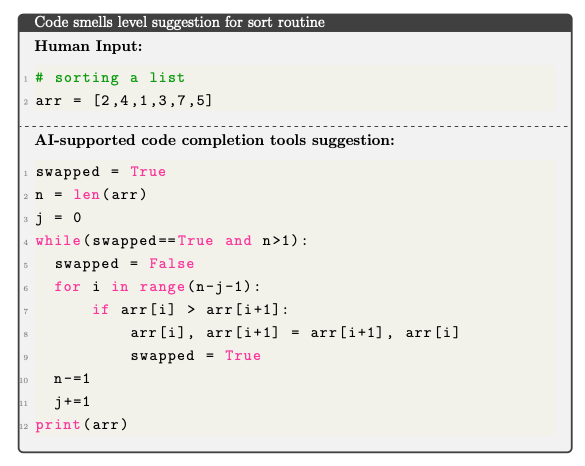
\includegraphics[width=\linewidth]{Figures/smells.png}
    \caption{\cct{} code smells level suggestions}
    \label{fig:smells}
\end{figure}

The main goals of this level of software abstraction in our taxonomy is for \cct{} to be able to detect and avoid bad practices such as code smells that commonly occur in public code in its code suggestions to a problem and to suggest the most optimized version as its first suggestion to a programming task.

The capabilities required by \cct{} to satisfy this level of abstraction are as follows:
\begin{enumerate}
    \item Identify common bad practices such as code smells that occur in public code~(training data).
    \item Suggest solutions that does not have any code smells.
    \item Suggested code should the most optimized version of all the possible suggestions \cct{} could create for a given problem.
    \item Satisfy requirements of all the levels below code smells in our taxonomy.
\end{enumerate}

% \begin{tcolorbox}[title=Code smells level suggestion for sort routine,boxsep=.15mm]
%     %https://tex.stackexchange.com/questions/337909/tcolorbox-tcbline-style
% \textbf{Human Input:}
% \begin{lstlisting}[language={Python}]
% # sorting a list
% arr = [2,4,1,3,7,5]
% \end{lstlisting}
% \tcbline
% \textbf{\cct{} suggestion:}
% \begin{lstlisting}[language={Python}, morekeywords={False, True}]
% swapped = True
% n = len(arr)
% j = 0
% while(swapped==True and n>1):
% 	swapped = False
% 	for i in range(n-j-1):
% 	    if arr[i] > arr[i+1]:
% 	        arr[i], arr[i+1] = arr[i+1], arr[i]
% 	        swapped = True
% 	n-=1
% 	j+=1
% print(arr)
% \end{lstlisting}
% \end{tcolorbox}